\documentclass[a4paper,12pt]{ujarticle}
\usepackage{listings,jlisting}
\usepackage[top=15truemm,bottom=15truemm,left=20truemm,right=20truemm]{geometry}
\usepackage[dvips]{graphicx}
\usepackage{siunitx}
\usepackage{multirow}
\usepackage{makecell}
\begin{document}
\title{マイクロコンピュータ 後期期末レポート}
\author{電気情報工学科2年 \\ E1533 西総一朗}
\date{2017年2月10日提出}
\maketitle
\begin{itemize}
 \item \large 光が流れるプログラム(片道バージョン)
 \item 光が流れるプログラム(往復バージョン)
 \item パルスモータ1-2相励磁プログラム
 \item 電子サイコロのプログラム
 \item タイマ割り込み制御プログラム
\end{itemize}
\clearpage
\tableofcontents
\clearpage
 \section{リスト5-5(光が流れるプログラム(片道バージョン))}
  \subsection{プログラム説明}
  8個あるLEDの内1個を左端から右へ0.5秒間隔で順次点灯することによって、光が流れるように見えるプログラム。
  \subsection{フローチャート}
  このプログラムのフローチャートを図\ref{fig:flow_5-5}に示す。
  \begin{figure}[htbp]
   \begin{center}
    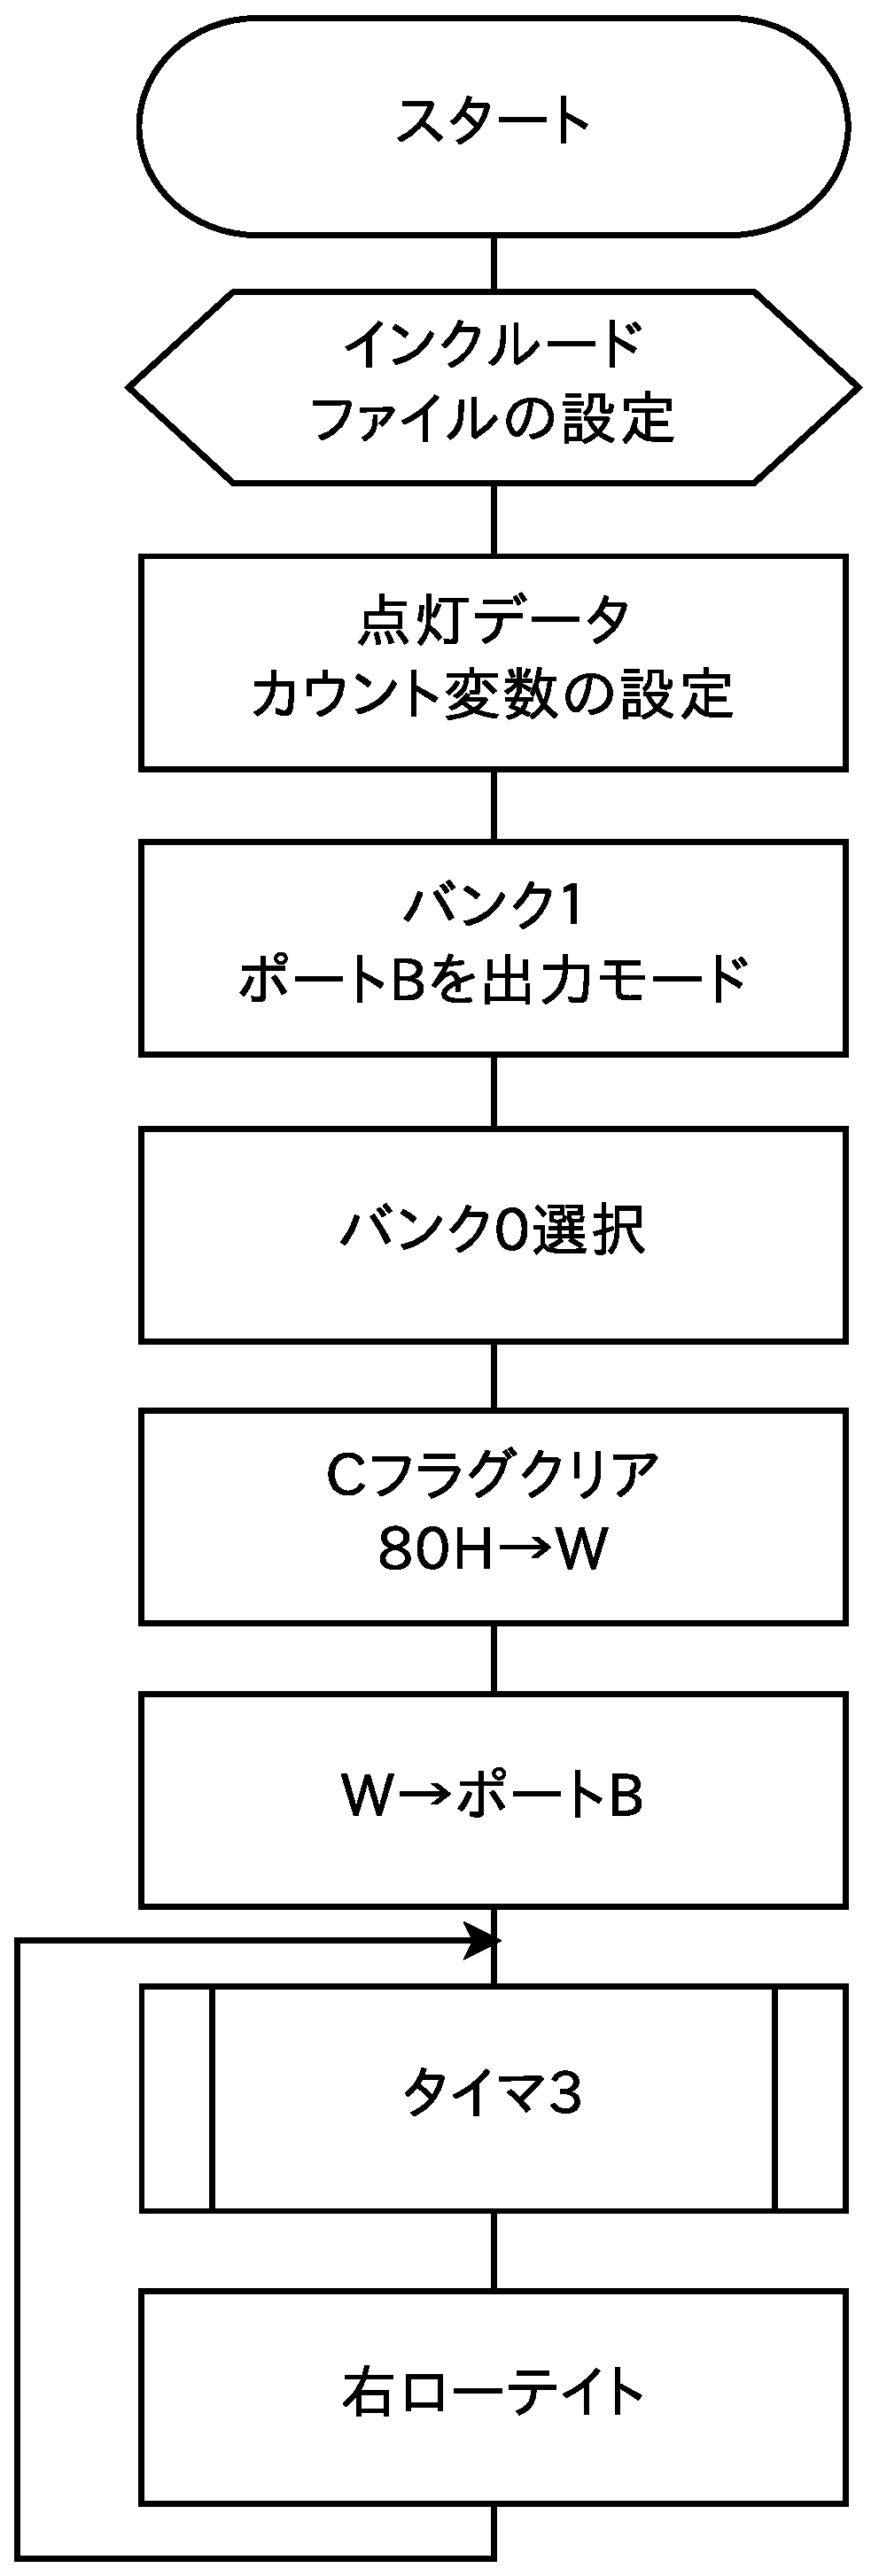
\includegraphics[height=185mm]{Diagram5-5.eps}
   \end{center}
   \caption{光が流れるプログラム ( 片道バージョン )のフローチャート}
   \label{fig:flow_5-5}
  \end{figure}
   \clearpage
  \subsection{ソースコード}
   \begin{lstinputlisting}[basicstyle=\ttfamily\footnotesize, frame=single,numbers=left]
    {../5-5/5-5.asm}
   \end{lstinputlisting}
   \clearpage
  \subsection{実行結果・考察}
   \begin{figure}[htbp]
    \begin{center}
     \begin{tabular}{c|cc}\hline
      状態&76543210 & C \\ \hline
      \multirow{2}{*}{1}&{80}$_{16}$ = 10000000$_2$ \\
      &●○○○○○○○ & □\\ \hline
      \multirow{2}{*}{2}&{40}$_{16}$ = 01000000$_2$ \\
      &○●○○○○○○ & □\\ \hline
      \multirow{2}{*}{3}&{20}$_{16}$ = 00100000$_2$ \\
      &○○●○○○○○ & □\\ \hline
      \multirow{2}{*}{4}&{10}$_{16}$ = 00010000$_2$ \\
      &○○○●○○○○ & □\\ \hline
      \multirow{2}{*}{5}&{08}$_{16}$  = 00001000$_2$ \\
      &○○○○●○○○ & □\\ \hline
      \multirow{2}{*}{6}&{04}$_{16}$  = 00000100$_2$ \\
      &○○○○○●○○ & □\\ \hline
      \multirow{2}{*}{7}&{02}$_{16}$  = 00000010$_2$ \\
      &○○○○○○●○ & □\\ \hline
      \multirow{2}{*}{8}&{01}$_{16}$  = 00000001$_2$ \\
      &○○○○○○○● & □\\ \hline
      \multirow{2}{*}{9}&{00}$_{16}$  = 00000000$_2$ \\
      &○○○○○○○○ & ■\\ \hline
     \end{tabular}\\
     ●:LED点灯 ○:LED消灯,■:Cフラグ1 □:Cフラグ0
    \end{center}
    \caption{光が流れるプログラム ( 片道バージョン )の実行結果。上の数字はポートBの値を表す。}
    \label{fig:out_5-5}
   \end{figure}
   図\ref{fig:out_5-5}はポートBの出力状態を表している。0.5秒毎にLEDの点灯箇所が右に移動していき(状態1〜9)、右端に到達する(状態9)と全てのLEDが消灯する。この一連の動作を繰り返す。ローテイト(RRF)命令はCフラグを経由してデータを1ビット右にシフトするのでCフラグにデータが存在するときには全てのLEDが消灯している。\\

   このプログラムのタイマについて考えてみる。
   PICのクロック周波数は$10\si{\mega\hertz}$なので、1クロックは
    \[
     \frac{1}{10\si{\mega\hertz}} = \SI{0.1}{\mu\second}
    \]
    4クロックで1サイクルなので、1サイクルは
    \[
     \SI{0.1}{\mu\second} \times 4 = \SI{0.4}{\mu\second}
    \]
     \begin{figure}[h]
      \begin{center}
       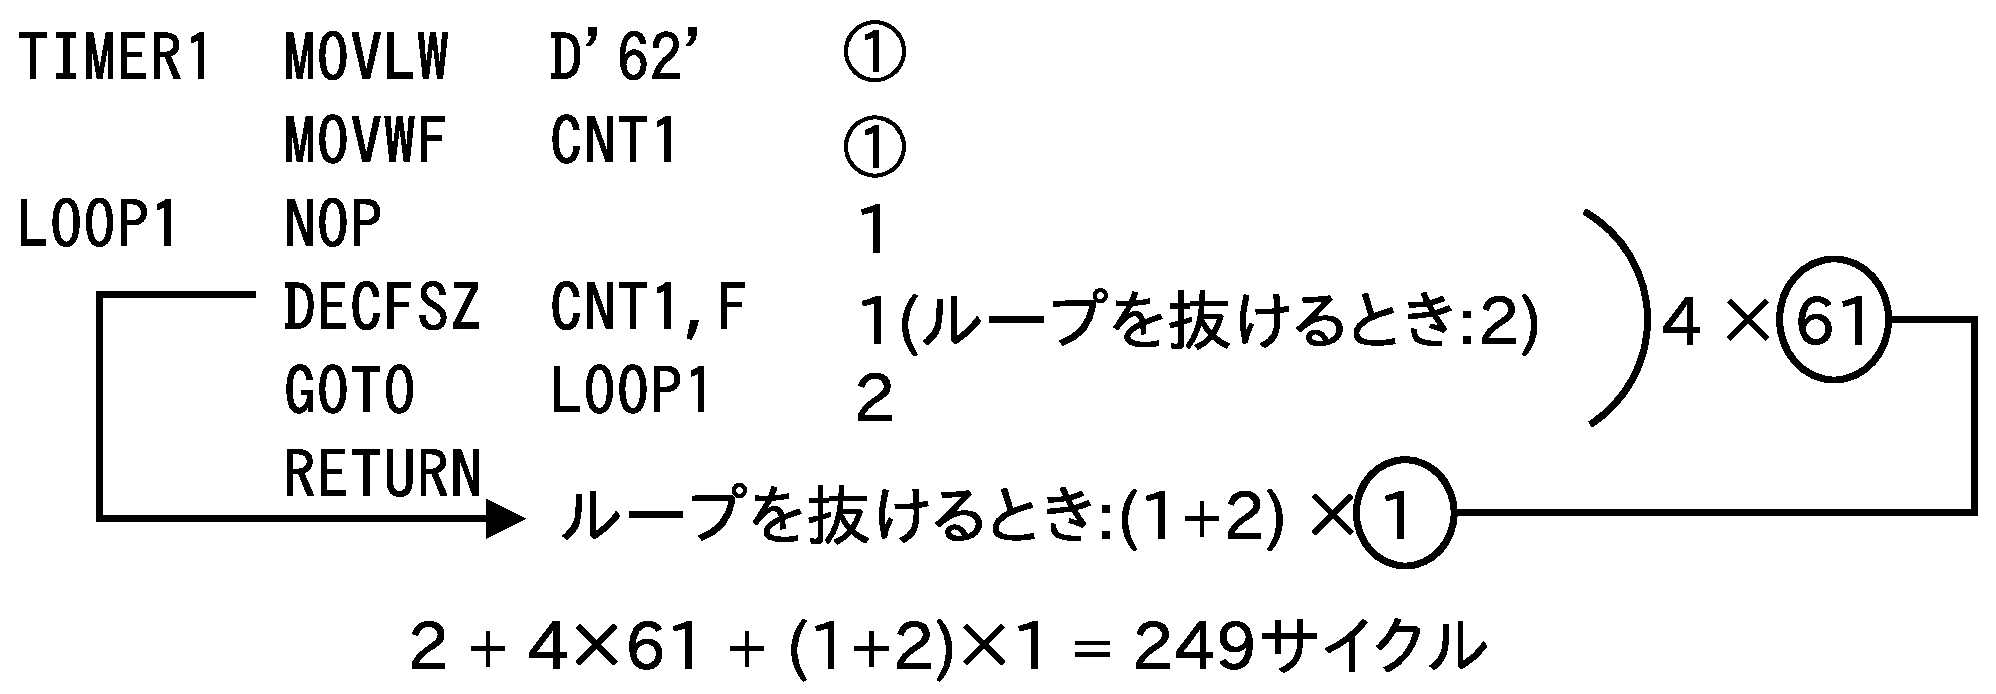
\includegraphics[width=130mm]{Diagram5.eps}
      \end{center}
      \caption{サイクル数の考え方}
      \label{fig:sicle}
     \end{figure}
     TIMER1のサイクル数は図\ref{fig:sicle}より、249サイクルだとわかり、
     \[
      \SI{0.4}{\mu\second} \times 249 = \SI{99.6}{\mu\second} \approx \SI{0.1}{\milli\second}
     \]
     TIMER1では$\SI{0.1}{\milli\second}$かかる。\\
     このTIMER1をTIMER2では100回呼び出し、TIMER3はTIMER2を50回呼び出しているので、
     \[
      \SI{0.1}{\milli\second} \times 100 \times 50 = \SI{50}{\milli\second} = \SI{0.5}{\second}
     \]
     よってTIMER1,TIMER2,TIMER3の合計で$\SI{0.5}{\second}$のタイマールーチンであることがわかる。\\

     次に光の移動方向について考えてみる。
     このプログラムにおいて、光の移動方向を決めているのは
      \begin{lstlisting}[basicstyle=\ttfamily\footnotesize, frame=single]
 9行目     LEDD    EQU     80H     ;LEDの点灯データの設定

24行目     RRF     PORTB,1         ;ポートBを1ビット右にローテイト
      \end{lstlisting}
      この2つなので次のように変更すれば左方向に移動するようになる。
      \begin{lstlisting}[basicstyle=\ttfamily\footnotesize, frame=single]
 9行目     LEDD    EQU     01H     ;LEDの点灯データの設定

24行目     RLF     PORTB,1         ;ポートBを1ビット右にローテイト
      \end{lstlisting}
      RLF命令もRRF命令と同様に、C フラグを経由してデータを 1 ビット左にシフトするので C フラグにデータが存在するときには全ての LED が消灯している。

      LEDの移動時間$S$を調整するにはTIMER1の0.1ミリ秒を基準にして、
      \begin{eqnarray*}
       S = \SI{0.1}{\milli\second} \times {\rm TIMER2 \times TIMER3} \\
       {\rm TIMER2 \le 255},\ {\rm TIMER3 \le 255}
      \end{eqnarray*}
      TIMER2とTIMER3とで移動時間$S$を調整する。
      \clearpage
 \section{リスト5-6(光が流れるプログラム(往復バージョン))}
  \subsection{プログラム説明}
  8個あるLEDの内1個を左端から右へ0.5秒間隔で順次点灯していき、右端に到達すると移動方向を逆にして左端に向かう。光が左から右へ流れるように見え、右端に到達すると右から左へ流れるように見えるプログラム。
  \subsection{フローチャート}
  このプログラムのフローチャートを図\ref{fig:flow_5-6}に示す。
  \begin{figure}[htbp]
   \begin{center}
    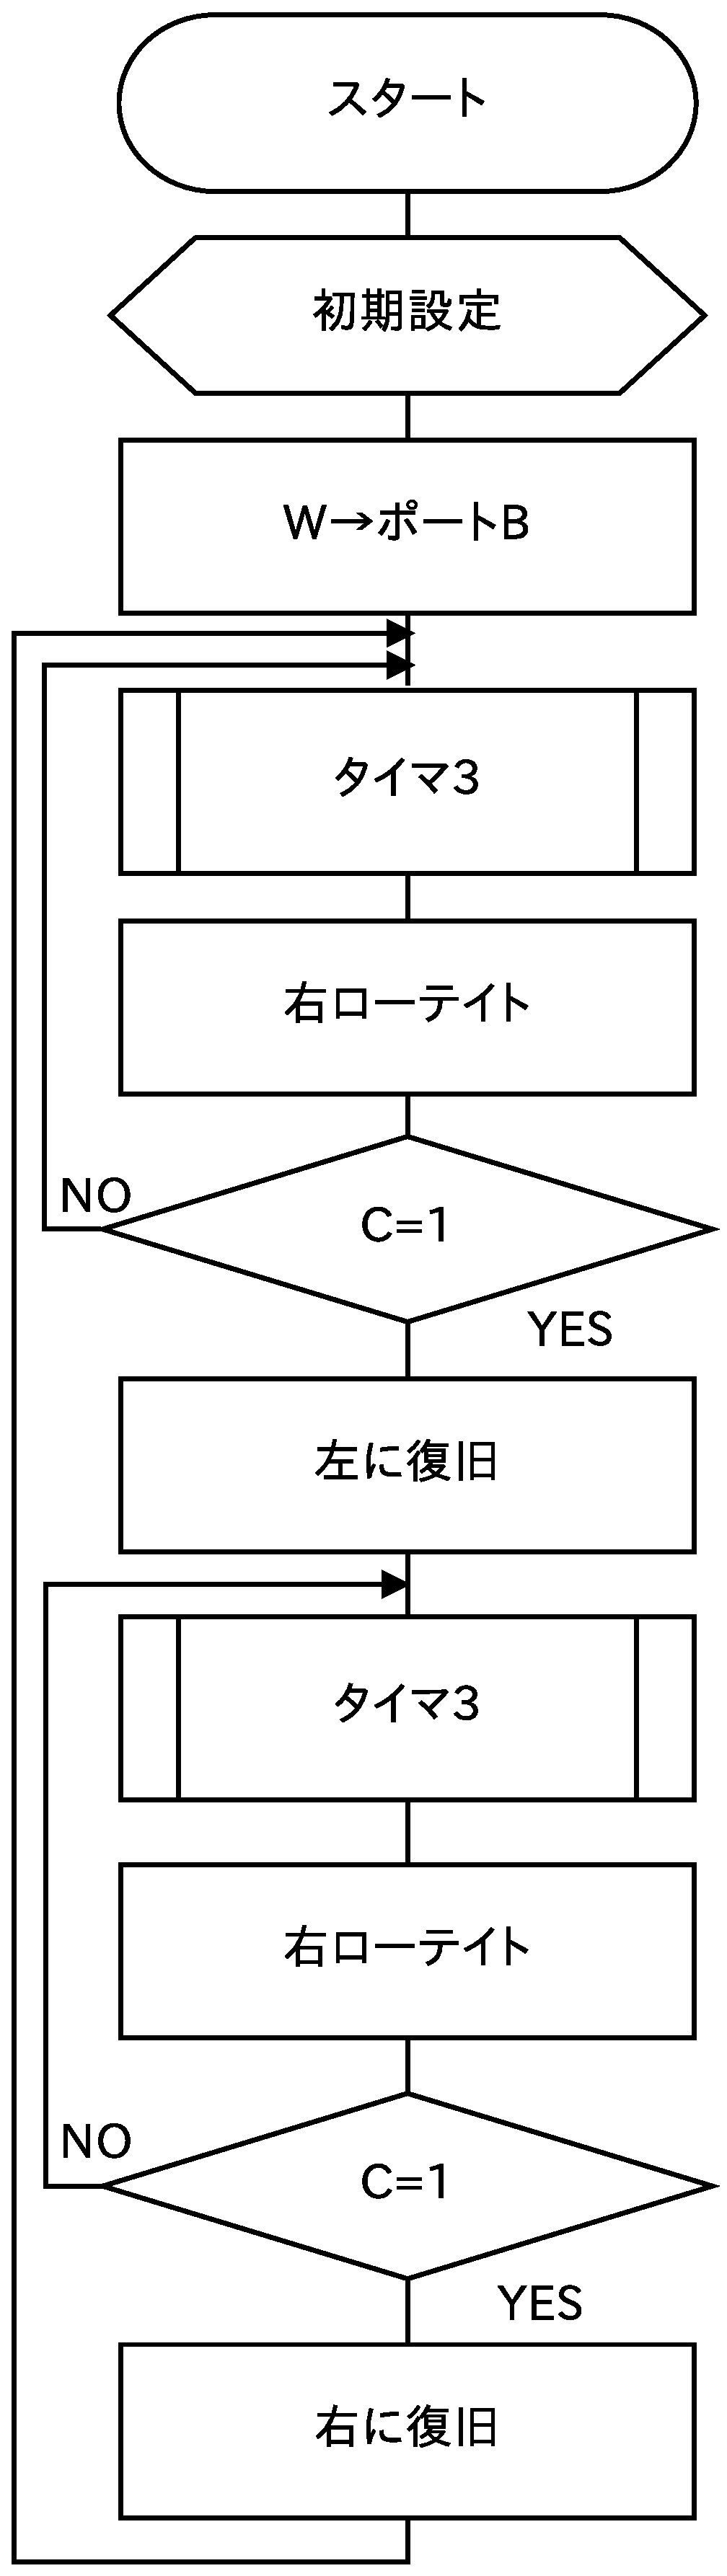
\includegraphics[height=180mm]{Diagram5-6.eps}
   \end{center}
   \caption{光が流れるプログラム ( 往復バージョン )のフローチャート}
   \label{fig:flow_5-6}
  \end{figure}
  \clearpage
  \subsection{ソースコード}
   \begin{lstinputlisting}[basicstyle=\ttfamily\footnotesize, frame=single,numbers=left]
    {../5-6/5-6.asm}
   \end{lstinputlisting}
  \subsection{実行結果・考察}
  \begin{figure}[htbp]
   \begin{center}
    \begin{tabular}{c|c||c|c}\hline
     状態&76543210       &状態 &76543210 \\ \hline
     \multirow{2}{*}{1}&{80}$_{16}$ = 10000000$_2$& \multirow{2}{*}{8}&{01}$_{16}$  = 00000001$_2$ \\
     &●○○○○○○○            & &○○○○○○○● \\ \hline
     \multirow{2}{*}{2}&{40}$_{16}$ = 01000000$_2$ & \multirow{2}{*}{9}&{02}$_{16}$  = 00000010$_2$ \\
     &○●○○○○○○            & &○○○○○○●○ \\ \hline
     \multirow{2}{*}{3}&{20}$_{16}$ = 00100000$_2$ & \multirow{2}{*}{10}&{04}$_{16}$  = 00000100$_2$ \\
     &○○●○○○○○            & &○○○○○●○○ \\ \hline
     \multirow{2}{*}{4}&{10}$_{16}$ = 00010000$_2$ & \multirow{2}{*}{11}&{08}$_{16}$  = 00001000$_2$ \\
     &○○○●○○○○            & &○○○○●○○○ \\ \hline
     \multirow{2}{*}{5}&{08}$_{16}$  = 00001000$_2$ &\multirow{2}{*}{12}& {10}$_{16}$ = 00010000$_2$ \\
     &○○○○●○○○            & &○○○●○○○○ \\ \hline
     \multirow{2}{*}{6}&{04}$_{16}$  = 00000100$_2$ &\multirow{2}{*}{13}& {20}$_{16}$ = 00100000$_2$ \\
     &○○○○○●○○            & &○○●○○○○○ \\ \hline
     \multirow{2}{*}{7}&{02}$_{16}$  = 00000010$_2$ &\multirow{2}{*}{14}&{40}$_{16}$ = 01000000$_2$ \\
     &○○○○○○●○            & &○●○○○○○○ \\ \hline
    \end{tabular}\\
     ●:LED点灯 ○:LED消灯
     \caption{光が流れるプログラム ( 往復バージョン )の実行結果。上の数字はポートBの値を表す。}
     \label{fig:out_5-6}
   \end{center}
  \end{figure}
   図\ref{fig:out_5-6}はポートBの出力状態を表している。
   0.2秒毎にLEDの点灯箇所が右に移動していき(状態1〜7)右端(状態8)に到達したら、移動方向を左に反転する(状態8〜14)。
   左端(状態1)に到達したら再びこの一連の動作を繰り返す。
   ローテイト(RRF,RLF)命令はCフラグを経由してデータを1ビット(右,左)にシフトするのでCフラグにデータが存在するかどうかで、
   光が右端(0ビット目)または左端(7ビット目)に移動したことを判定している。
   Cフラグが1の場合はオーバーフローかアンダーフローしているので、
   図\ref{fig:under}に過分ローテートの復旧を示す。状態9の次に状態Uがくるが、
   状態Uに到達したらすぐに過分ローテートの復旧するためにRLF命令を2回実行することで、状態10に移行し光がなめらかに移動するように見える。

   \begin{figure}[htbp]
    \begin{center}
      \begin{tabular}{c|cc|l}\hline
      状態&76543210 & C  &\makecell[c]{説明} \\ \hline
      \multirow{2}{*}{9}&{01}$_{16}$ = 00000001$_2$ && \multirow{2}{*}{0ビット目点灯} \\
      &○○○○○○○● & □ & \\ \hline
      \multirow{2}{*}{U}&{00}$_{16}$ = 00000000$_2$ && \multirow{2}{*}{Cフラグにアンダーフロー} \\
      &○○○○○○○○ & ■ & \\ \hline
      \multirow{2}{*}{10}&{02}$_{16}$ = 00000010$_2$&& \multirow{2}{*}{過分ローテート復旧(RLF $\times$ 2)} \\
      &○○○○○○●○ & □ & \\ \hline
      \end{tabular}\\
     ●:LED点灯 ○:LED消灯,■:Cフラグ1 □:Cフラグ0
     \caption{過分ローテート復旧の例。上の数字はポートBの値を表す。}
     \label{fig:under}
    \end{center}
   \end{figure}
   光の移動方向については、Cフラグでの判定と過分ローテートの復旧を行っているため、LEDの点灯データを変えるだけで、移動方向を変えられる。プログラムの9行目
   \begin{lstlisting}[basicstyle=\ttfamily\footnotesize, frame=single]
9行目    LEDD     EQU     80H    ;左端から右方向にスタート
   \end{lstlisting}
   を次のように変更すれば、スタート時の移動方向を反対にできる。
   \begin{lstlisting}[basicstyle=\ttfamily\footnotesize, frame=single]
9行目    LEDD     EQU     01H    ;右端から左方向にスタート
   \end{lstlisting}

   \vspace{3mm}

   次に過分ローテイトの復旧がない場合について考えてみる。
    \begin{figure}[htbp]
     \begin{center}
      \begin{tabular}{c|cc|l}\hline
       状態&76543210 & C  &\makecell[c]{説明}\\ \hline
       \multirow{2}{*}{7}&{02}$_{16}$ = 00000010$_2$ && \multirow{2}{*}{1ビット目点灯} \\
       &○○○○○○●○ & □ & \\ \hline
       \multirow{2}{*}{8}&{01}$_{16}$ = 00000001$_2$ && \multirow{2}{*}{0ビット目点灯} \\
       &○○○○○○○● & □ & \\ \hline
       \multirow{2}{*}{U}&{00}$_{16}$ = 00000000$_2$ && \multirow{2}{*}{Cフラグにアンダーフロー} \\
       &○○○○○○○○ & ■ & \\ \hline
       \multirow{2}{*}{8}&{01}$_{16}$ = 00000001$_2$ && \multirow{2}{*}{0ビット目点灯} \\
       &○○○○○○○● & □ & \\ \hline
       \multirow{2}{*}{9}&{02}$_{16}$ = 00000010$_2$ && \multirow{2}{*}{1ビット目点灯} \\
       &○○○○○○●○ & □ & \\ \hline
      \end{tabular}\\
      ●:LED点灯 ○:LED消灯,■:Cフラグ1 □:Cフラグ0
      \caption{過分ローテート復旧がない場合。上の数字はポートBの値を表す。}
      \label{fig:under_less}
     \end{center}
    \end{figure}

    図\ref{fig:under_less}のように過分ローテイトの復旧がないと、全てのLEDが0.5秒間点灯しないので不自然に移動してるように見える。
    \clearpage
 \section{リスト 5-12(パルスモータ 1-2 相励磁プログラム)}
  \subsection{プログラム説明}
    1相励磁と2相励磁を交互に繰り返して、パルスモータを制御するプログラム。
    時計回りに配置されている4つのコイル$X$,$Y$,$\bar{X}$,$\bar{Y}$について順に電流を流していく。
    4つのコイル$X$,$Y$,$\bar{X}$,$\bar{Y}$はこの順に$90^\circ$ずつ配置されている。
    励磁の順序は最初に$X$、次に$X$と$Y$、次に$Y$のように行う。
    すなわち、コイルを1つ励磁し、次に隣のコイルと合わせて2つ励磁し、次に隣のコイル1つだけを励磁するのを繰り返す。
    この動作をまとめると表\ref{table:1-2}になる。表\ref{table:1-2}の$X$,$Y$,$\bar{X}$,$\bar{Y}$の組をデータとして予めファイルレジスタに入れておいて、これらを順に呼び出して出力する。
    \begin{table}[h]
     \begin{center}
      \caption{1-2相励磁の場合のコイルに流す電流の組の順序}
      \label{table:1-2}
      \vspace{2mm}
      \begin{tabular}[h]{|c||c|c|c|c|c|c|c|c|}\hline
       &1&2&3&4&5&6&7&8 \\ \hline \hline
       $X$&1&1&0&0&0&0&0&1 \\
       $Y$&0&1&1&1&0&0&0&0 \\
       $\bar{X}$&0&0&0&1&1&1&0&0 \\
       $\bar{Y}$&0&0&0&0&0&1&1&1 \\ \hline \hline
      データ &$8_{16}$&$C_{16}$&$4_{16}$&$6_{16}$&$2_{16}$&$3_{16}$&$1_{16}$&$9_{16}$ \\ \hline
      \end{tabular}
     \end{center}
    \end{table}
  \subsection{フローチャート}
    図\ref{fig:flow_5-12}にこのプログラムのフローチャートを示す。
  \subsection{ソースコード}
    \begin{lstinputlisting}[basicstyle=\ttfamily\footnotesize, frame=single,numbers=left]
     {../5-12/5-12.asm}
    \end{lstinputlisting}

    \begin{figure}[htbp]
     \begin{center}
      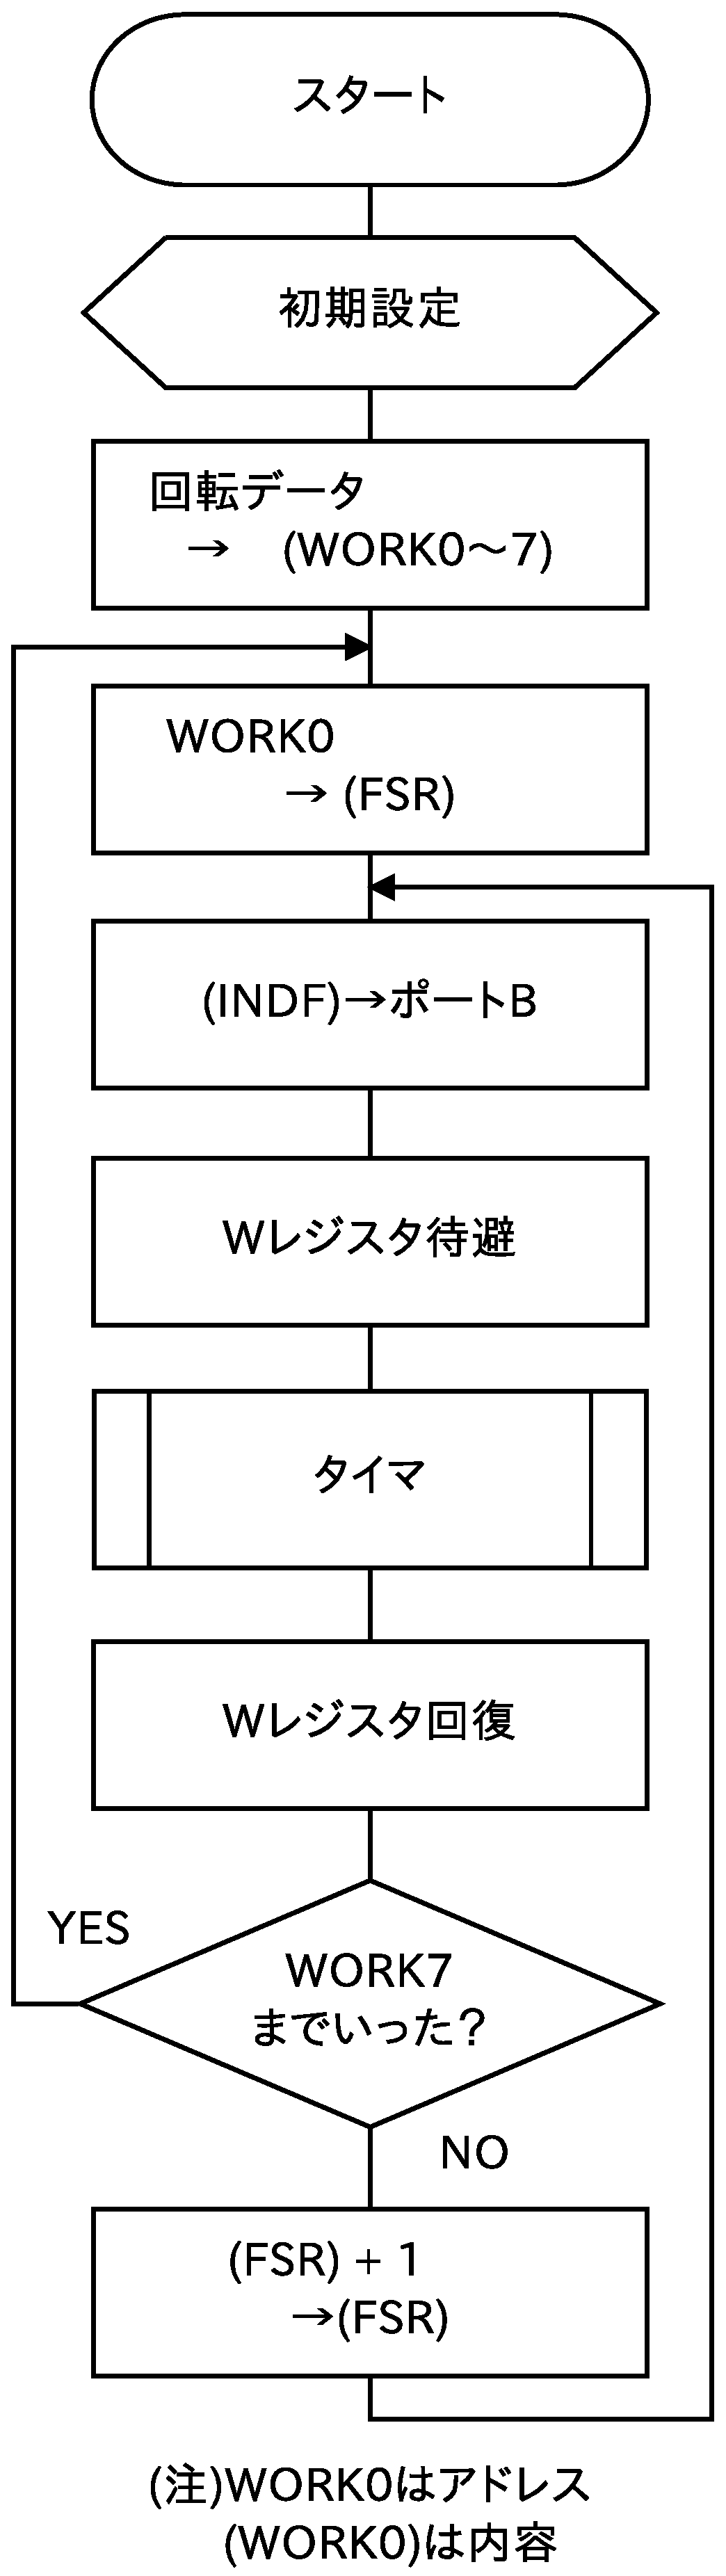
\includegraphics[height=230mm]{Diagram5-12.eps}
     \end{center}
     \caption{パルスモータ 1-2 相励磁プログラムのフローチャート}
     \label{fig:flow_5-12}
    \end{figure}
    \subsection{実行結果・考察}
    実行する前にボードのRB0をDOWNにスイッチしておく。実験で使用したボードにはパルスモータが接続されていないのでLEDで動作を確認する。
    \begin{figure}[htbp]
     \begin{center}
       \begin{tabular}{c|c|c}\hline
        \multirow{2}{*}{状態}&76543210 & \multirow{2}{*}{データ}\\
        &    $X$\,$Y$\,$\bar{X}$\,$\bar{Y}$\\ \hline
         1&○○○○●○○○ & $8_{16}=00001000_2$ \\
         2&○○○○●●○○ & C$_{16}=00001100_2$\\
         3&○○○○○●○○ & $4_{16}=00000100_2$\\
         4&○○○○○●●○ & $6_{16}=00000110_2$\\
         5&○○○○○○●○ & $2_{16}=00000010_2$\\
         6&○○○○○○●● & $3_{16}=00000011_2$\\
         7&○○○○○○○● & $1_{16}=00000001_2$\\
         8&○○○○●○○● & $9_{16}=00001001_2$\\ \hline
       \end{tabular}\\
      ●:LED点灯 ○:LED消灯
      \caption{パルスモータ 1-2 相励磁プログラムの実行結果}
      \label{fig:out_5-12}
     \end{center}
    \end{figure}

    図\ref{fig:out_5-12}はポートBの出力状態を表している。8個のLEDの内右側の4つが
    それぞれコイル$X$,$Y$,$\bar{X}$,$\bar{Y}$に対応している。
    状態1〜8はLEDの点灯状態で、0.5秒毎に移行していく。状態8の次は状態1に戻る。
    各コイルでみると対応するLEDが1.5秒点灯して、2.5秒消灯するように変化している。
    各コイルの動作は1秒ずれているので、1相励磁と2相励磁が交互に繰り返す様子が確認できた。

    この動作を実現するためにあらかじめデータをメモリに入れておいて、それを読みだしてPORTBにセットしている。
    FSRレジスタの内容を1ずつ変えて、INDFレジスタを読みだすと
    FSRレジスタの内容が指すメモリアドレスにアクセスすることで読み出しを実現している。
    つまり間接アドレッシング方式を用いている。

    読みだす順序を変えるだけで、モーターを反転させることができる。
    そのためには読みだす最初のアドレスを反対からにして読みだすアドレスを1つずつ減らしていく。
     \begin{lstlisting}[basicstyle=\ttfamily\footnotesize, frame=single]
47行目      NEW  MOVLW  WORK0
54行目           SUBWF  WORK7
58行目           INCF   FSR,F
     \end{lstlisting}
     このコードを
     \begin{lstlisting}[basicstyle=\ttfamily\footnotesize, frame=single]
47行目      NEW  MOVLW  WORK7
54行目           SUBWF  WORK0
58行目           DECF   FSR,F
     \end{lstlisting}
     このように変えるとよい。

     回転の速さはTIMER3のカウント数で調整すればよい。
     \\

     1相制御にするにはWORK0〜WORK7に格納するデータを
     \begin{table}[htbp]
      \begin{center}
       \caption{1相励磁のデータ}
       \label{table:1-data}
       \begin{tabular}{|c|c|}
        \hline
        WORK0 & 08$_{16}=00001000_2$\\
        WORK1 & 04$_{16}=00000100_2$\\
        WORK2 & 02$_{16}=00000010_2$\\
        WORK3 & 01$_{16}=00000001_2$\\ \hline
       \end{tabular}
      \end{center}
     \end{table}
     表\ref{table:1-data}のようにして、WORK5〜WORK7は使わず、コードの54行目を
     \begin{lstlisting}[basicstyle=\ttfamily\footnotesize, frame=single]
54行目           SUBWF  WORK3
     \end{lstlisting}
     のように変えれば良い。
     \\

     2相制御なら、同様に表\ref{table:2-data}のデータを与えればよい。
     \begin{table}[htbp]
      \begin{center}
       \caption{2相励磁のデータ}
       \label{table:2-data}
       \begin{tabular}{|c|c|} \hline
        WORK0 & 0C$_{16}=00001100_2$\\
        WORK1 & 06$_{16}=00000110_2$\\
        WORK2 & 03$_{16}=00000011_2$\\
        WORK3 & 09$_{16}=00001001_2$\\ \hline
       \end{tabular}
      \end{center}
     \end{table}

     このようにテーブルを与えて順に読みだす方式は非常に汎用的な制御方法と考えられる。
\end{document}
